\documentclass{beamer}
\usetheme{Madrid}
\usepackage[spanish]{babel}
\usepackage{amsmath}
\usepackage{caption}
\usepackage{ragged2e}  
\usepackage{multicol}
\captionsetup[figure]{font=scriptsize}
\setbeamertemplate{caption}[numbered]





% Paquete para posicionar el logo
\usepackage[absolute,overlay]{textpos} 

% Paquete para importar imágenes
\usepackage{graphicx}  

\setbeamertemplate{frametitle}{
  \begin{beamercolorbox}[sep=0.3cm,center,wd=\paperwidth]{frametitle}
    \usebeamerfont{frametitle}\parbox[c][0.8cm][c]{.8\textwidth}{\insertframetitle}\hfill
    \raisebox{-0.3\height}{
\includegraphics[height=0.8cm]{Logos/MarcaBlanco.png}}
  \end{beamercolorbox}
}


\def\supervisor{Dr. Carlos Fuhrhop}
\def\course{Control Avanzado}

\title{Control GPC en un motor DC}
\author{Ing. Rodrigo Salazar, Ing. Elvin Soto}
\institute{UACH}
\date{\today}

% Modificación de la planilla del titulo
\setbeamertemplate{title page}{
  \vbox{}
  \vfill
  \begin{centering}
    %Para llamar a los diferentes logotipos del titulo
    
\includegraphics[height=1.1cm]{Logos/electronica-color.png} \hspace{0.8cm}  
    
\includegraphics[height=1.5cm]{Logos/UACh_Marcacolor.png} \hspace{0.5cm} 
    
\includegraphics[height=0.9cm]{Logos/MarcaColor.png}  
    \par
    \vskip1.5em%
    {\usebeamercolor[fg]{titlegraphic}\inserttitlegraphic\par}
    \begin{beamercolorbox}[sep=8pt,center,colsep=-4bp,rounded=true,shadow=true]{title}
      \usebeamerfont{title}\inserttitle\par%
      \ifx\insertsubtitle\@empty%
      \else%
        \vskip0.25em%
        {\usebeamerfont{subtitle}\usebeamercolor[fg]{subtitle}\insertsubtitle\par}%
      \fi%     
    \end{beamercolorbox}%
    \vskip1em\par
    \begin{beamercolorbox}[sep=8pt,center,colsep=-4bp,rounded=true,shadow=true]{author}
      \usebeamerfont{author}\insertauthor
    \end{beamercolorbox}
    \begin{beamercolorbox}[sep=8pt,center,colsep=-4bp,rounded=true,shadow=true]{author}
      \usebeamerfont{author}Profesor: \supervisor
    \end{beamercolorbox}
    \begin{beamercolorbox}[sep=8pt,center,colsep=-4bp,rounded=true,shadow=true]{author}
        \usebeamerfont{author}Curso: \course
    \end{beamercolorbox}
    \begin{beamercolorbox}[sep=8pt,center,colsep=-4bp,rounded=true,shadow=true]{institute}
      \usebeamerfont{institute}\insertinstitute
    \end{beamercolorbox}
    \begin{beamercolorbox}[sep=8pt,center,colsep=-4bp,rounded=true,shadow=true]{date}
      \usebeamerfont{date}\insertdate
    \end{beamercolorbox}\vskip0.5em
    {\usebeamercolor[fg]{titlegraphic}\inserttitlegraphic\par}
    \par
    \vfill
  \end{centering}
}

\begin{document}
\begin{frame}
  \titlepage
\end{frame}


\begin{frame}
  \frametitle{Introducción}
  \frametitle{Modelo Motor DC}
  \frametitle{Control Predictivo GPC}
  \tableofcontents
\end{frame}

\section{Introducción}
\begin{frame}{Introducción}
\begin{justify}
\vspace{0.3cm}
\begin{itemize}
  El control de un motor de corriente continua (DC) se realiza con el objetivo de controlar su velocidad, dirección y/o par motor a partir de una entrada que generalmete es una fuente de voltaje [1]. Estos motores son ampliamente utilizados en diversas aplicaciones debido a su capacidad para ofrecer un control preciso sobre estos parámetros. 
  \\
  En este trabajo, nos enfocaremos en una estrategia de control predictivo específica conocida como Control Predictivo Generalizado (GPC, por sus siglas en inglés) para controlar la velocidad angular en función del voltaje.
\end{itemize}
\end{justify}
\end{frame}

\section{Modelo Motor DC}
\begin{frame}{Modelo Motor DC}
\begin{justify}
\vspace{0.3cm}
\begin{itemize}
El motor de corriente directa (DC) ha sido usado por muchos años como un convertidor básico de energía, es decir, convierte energía electrica en energía mecánica [2]. Estos motores son usados en procesos industriales como elevadores eléctricos, laminadores, vehículos eléctricos y algunas bombas donde se requiere de velocidad variable
\end{itemize}
\end{justify}
\end{frame}

\begin{frame}{Modelo Motor DC}
\begin{justify}
\vspace{0.3cm}
\begin{itemize}
\begin{figure}[h]
    \centering
    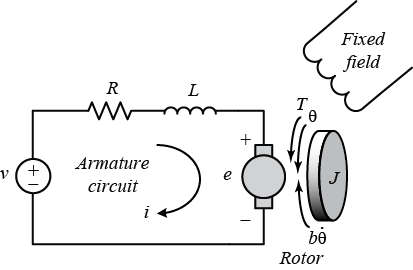
\includegraphics[width=0.7\linewidth]{motor.png}
    \caption{Esquema de un circuito de motor DC}
    \label{fig:enter-label}
\end{figure}
\end{itemize}
\end{justify}
\end{frame}

\begin{frame}{Modelo Motor DC}
\begin{justify}
\vspace{0.3cm}
\begin{itemize}
    El motor DC se modela con una resistencia constante R en serie con una inductancia constante L que representa la inductancia de la bobina del rotor, una caída de tensión $e_a$ en el rotor y una fuente de alimentación $v$.

Si se realiza una malla en el circuito se obtiene lo siguiente:
\begin{align}
v(t) &= Ri(t) + L\frac{di(t)}{dt}+E_a (t), 
\end{align}
Despejando para $L\frac{di(t)}{dt}$ queda:
\begin{align}
 L\frac{di(t)}{dt} &= v(t)-Ri(t) - E_a (t), 
\end{align}
\end{itemize}
\end{justify}
\end{frame}

\begin{frame}{Modelo Motor DC}
\begin{justify}
\vspace{0.3cm}
\begin{itemize}  
    Las pérdidas por fricción y parte de la energía es convertida a energía cinética rotacional en el rotor. La ecuación de la sección mecánica viene dada por el modelo:
\begin{equation*}
    T_m(t) = J\frac{d\omega(t)}{dt}+B\omega(t), 
\end{equation*}
\\
Despejando para $J\frac{d\omega(t)}{dt}$ queda:
\begin{align}
 J\frac{d\omega(t)}{dt} &= T_m(t)-B\omega(t), 
\end{align}
    Donde $T_m(t)$ es el torque del motor de corriente continua, $B$ es el coeficiente de fricción equivalente al motor de CD y la carga montados sobre el eje del motor, J es el momento de inercia total del rotor y de la carga con relación al eje del motor, $\omega(t)$ es la velocidad angular del motor y $\dfrac{d\omega(t)}{dt}$ es la aceleración angular.
\end{itemize}
\end{justify}
\end{frame}



\begin{frame}{Modelo Motor DC}
\begin{justify}
\vspace{0.3cm}
\begin{itemize}  
Para poder lograr la interacción entre las ecuaciones anteriores se proponen las siguientes relaciones que asumen que existe una relación proporcional, $K_a$ (Constante de fuerza contraelectromotriz $[v/rad s]$), entre el voltaje inducido en la armadura y la velocidad angular del eje del motor.

\begin{align}
E_a(t) &= K_a\omega(t),
\end{align}

Y se supone la siguiente relación electromecánica que establece que el torque mecánico es proporcional, $K_m$ (Constante de Torque $[Nm / A]$), a la corriente eléctrica que circula por el motor DC.

\begin{align}
T_m(t) &= K_m i(t),
\end{align}

\end{itemize}
\end{justify}
\end{frame}

\begin{frame}{Modelo Espacio-Estado}
\begin{justify}
\vspace{0.3cm}
\begin{itemize}  
   Definimos los estados como:
    \begin{align}
        x_1&=\omega \\
        \dot{x}_1&=\dot{\omega} \\
        x_2&=i \\
        \dot{x}_2&=\dot{i} 
    \end{align}

Reescribiendo las ecuaciones se tiene:

\begin{align}
    \dot{x}_1&=-\frac{B}{J}x_1+\frac{K_m}{J}x_2 \\
    \dot{x}_2&=-\frac{R}{L}x_2+\frac{K_a}{L}x_1+\frac{1}{L}v
\end{align}
\end{itemize}
\end{justify}
\end{frame}

\begin{frame}{Parámetros importantes motor DC}
\begin{justify}
\vspace{0.3cm}
\begin{itemize}  
\begin{table}[htbp]
    \centering
    \caption{Parámetros del motor DC}
    \begin{tabular}{|c|c|c|c|c|c|}
        \hline
        Momento de inercia del rotor (J) & 0.01 $kg.m^2$ \\
        \hline
        Constante de amortiguamiento del motor & 0.1 N.m.s  \\
        \hline
        Constante de rotor FEM ($K_c$) & 0.01 V/rad/sec  \\
        \hline
        Constante de torque-motor ($k_t$) & 0.01 N.m/Amp \\
        \hline
        Resistencia de rotor (R) & 1 Ohm \\
        \hline
         Inductancia de rotor (L) & 0.5 H \\
        \hline
    \end{tabular}
\end{table}
*FEM: Fuerza electromotriz
\end{itemize}
\end{justify}
\end{frame}

\begin{frame}{Modelo Motor DC}
\begin{justify}
\vspace{0.3cm}
\begin{itemize}  
  
La representación del modelo del motor DC en espacio estado de forma matricial es:
\[
\begin{bmatrix}
    \dot{x}_1 \\
    \dot{x}_2 \\
\end{bmatrix}
=
\begin{bmatrix}
    -\frac{B}{J} & \frac{K_m}{J} \\
    -\frac{K_a}{L} & -\frac{R}{L} \\
\end{bmatrix}
\begin{bmatrix}
    x_1 \\
    x_2 \\
\end{bmatrix}
+
\begin{bmatrix}
    0 \\
    \frac{1}{L} \\
\end{bmatrix} v
\]
\\
Reemplazando el modelo con los parámetros del cuadro 1 queda:
\[
\begin{bmatrix}
    \dot{x}_1 \\
    \dot{x}_2 \\
\end{bmatrix}
=
\begin{bmatrix}
    -10 & 1 \\
    -0.02 & -2 \\
\end{bmatrix}
\begin{bmatrix}
    x_1 \\
    x_2 \\
\end{bmatrix}
+
\begin{bmatrix}
    0 \\
    2 \\
\end{bmatrix} v
\]

\end{itemize}
\end{justify}
\end{frame}

\section{Control Predictivo GPC}
\begin{frame}{Control Predictivo GPC}
\begin{justify}

Hay tres componentes principales en el diseño de un GPC [3]:
\begin{itemize}


    \vspace{0.3cm}
    \item Un modelo lineal del sistema a controlar: Este modelo se utiliza para predecir la salida del sistema durante el horizonte de predicción.
    
    \vspace{0.3cm}
    \item Formulación de la función criterio.
    
    \vspace{0.3cm}
    \item Minimización de la función de criterio para producir la secuencia de salida de control óptima durante el horizonte de predicción.

\end{itemize}
\end{justify}
\end{frame}

\begin{frame}{Control Predictivo GPC}
\begin{justify}
Considera una ecuación descrita por el sistema de estado lineal:

\vspace{0.3cm}
   $$x(t+1)=Ax(t)+Bu(t)$$
   $$y(t)=Hx(t)$$
   
\vspace{0.2cm}
Donde $x(t) \in R^n,$ $y(t) \in R^r$ y $u(t) \in R^m$ son el estado y A, B y H son matrices con dimensiones apropiadas. La estructura de este modelo es usado para formular controles predictivos. Primero se define un modelo de predicción de estado de la forma:

\vspace{0.3cm}
$\hat{x}(t+j/t)=A\hat{x}(t+j-1/t)+Bu(t+j-1/t),$ $j=1. 2. ....., p, $ 

\vspace{0.3cm}
Siendo $\hat{x}(t+j/t)$ denota el vector de predicción en el instante t para  el instante t+j h(./t) denota la secuencia del control de vectores en el intervalo de prediccion. 

\end{justify}
\end{frame}

\begin{frame}{Control Predictivo GPC}
\begin{justify}


Este modelo es redefinido para cada instante de muestra t  del actual estado de vector y el control previamente aplicado.

$$\hat{x}(t/t)=x(t); u(t-j/t)=u(t-j); j=1,2,...,h.$$

\vspace{0.3cm}
Aplicando la ecuación anterior recursivamente a las condiciones iniciales, las siguientes ecuaciones pueden ser obtenidos:

$$\hat{y}(t+1/t)= HAx(t)+HBu(t)$$

$$\hat{y}(t+2/t)= HA^2x(t)+HABu(t)+HBu(t+1),$$

$$\hat{y}(t+p_1/t)=HA^{p_1}x(t)+HA^{p_{1}-1}Bu(t)+...+HA^{p_{1}-p_{2}-1}Bu(t+p_2)$$

Siendo $p_1$ y $p_2$ valores enteros positivos
\end{justify}
\end{frame}



\begin{frame}{Control Predictivo GPC}
\begin{justify}
\begin{itemize}
Una forma reducida de escribir esta ecuación es de la siguiente manera:
$Y=Gx(t)+F_1 U$
\\ 

\vspace{0.3cm}
Donde:
\centering
\hfill \break
$Y=\begin{bmatrix}\hat{y}(t+1/t) &\hat{y}(t+2/t)&...& \hat{y}(t+p_1/t)
\end{bmatrix} ^T$
\\
\hfill \break
\\
$G=
\begin{bmatrix}
    HA \\
    HA^2\\
    . \\
    .\\
    HA^{p_1}
\end{bmatrix}$,
$F_1=
\begin{bmatrix}
    HB & 0 & ... & 0 \\
    HAB & HB & ... & 0\\
    . & . & ... & . \\
    . & . & ... & . \\
    . & . & ... & . \\
    HA^{p_1-1} & HA^{p_1-2}B & ... & HA^{p_1-p_2-1}B
\end{bmatrix}
$
\\
\hfill \break
\\
$U=\begin{bmatrix}u(t)& u(t+1)&...& u(t+p_2)\end{bmatrix}^T$ 
\\

\end{itemize}
\end{justify}
\end{frame}



\begin{frame}{Función objetivo sin penalización en la acción de control:}
\begin{justify}

La ley de control predictivo generalmente se formula para minimizar una función de costos, también llamada criterio de desempeño.

\vspace{0.3cm}
Un criterio de desempeño simple que se puede utilizar en el diseño de control predictivo está dado por:

\vspace{0.3cm}
\begin{itemize}
    \item \( J = \frac{1}{2} \sum_{j=1}^{p1} \left( y_d(t + j) - \hat{y}(t + j) \right)^T Q_j \left( y_d(t + j) - \hat{y}(t + j) \right) \)

    \vspace{0.3cm}
    o
    
    \vspace{0.3cm}
    \item \( J = \frac{1}{2} (Y_d - Y)^T Q (Y_d - Y) \)
\end{itemize}

\vspace{0.3cm}
Esta función objetivo solo considera el error entre la salida deseada \( y_d \) y la salida predicha \( \hat{y} \) del sistema, \( Q \) es una matriz de ponderación (o peso) que determina cuánto se penaliza la desviación en la predicción de la salida del sistema.

\end{justify}
\end{frame}

\begin{frame}{Control Predictivo GPC}
\begin{justify}

Función objetivo con penalización en la acción de control:

\vspace{0.3cm}
\begin{itemize}
    \item \( J = \frac{1}{2} \sum_{j=1}^{p1} \left( y_d(t + j) - \hat{y}(t + j) \right)^T Q_j \left( y_d(t + j) - \hat{y}(t + j) \right) + \frac{1}{2} \sum_{j=0}^{p2} u(t + j)^T R_j u(t + j) \)
    
    \vspace{0.3cm}
    o
    
    \vspace{0.3cm}
    \item \( J = \frac{1}{2} (Y_d - Y)^T Q (Y_d - Y) + U^T R U \)
\end{itemize}

\vspace{0.3cm}
Esta versión de la función objetivo añade un término adicional para penalizar la magnitud de la acción de control \( u \). Aquí, \( R \) es una matriz de ponderación que determina cuánto se penaliza la acción de control.


\end{justify}
\end{frame}

\begin{frame}{Función objetivo con penalización en la acción de control }
\begin{justify}

Función objetivo con penalización en el cambio de la acción de control:


\vspace{0.3cm}
\begin{itemize}
    \item \( J = \frac{1}{2} \sum_{j=1}^{p1} \left( y_d(t + j) - \hat{y}(t + j) \right)^T Q_j \left( y_d(t + j) - \hat{y}(t + j) \right) + \frac{1}{2} 
    \sum_{j=0}^{p2} \Delta u(t + j)^T R_j \Delta u(t + j) \)

    \vspace{0.3cm}
    o
    
    \vspace{0.3cm}
    \item \( J = \frac{1}{2} (Y_d - Y)^T Q (Y_d - Y) + \Delta U^T R \Delta U \)
\end{itemize}

\vspace{0.3cm}
Esta función objetivo es similar a la anterior, pero en lugar de penalizar la magnitud de la acción de control, penaliza los cambios en la acción de control \( \Delta u \). Esto se hace para suavizar la trayectoria de la acción de control, evitando cambios bruscos de un paso a otro.


\end{justify}
\end{frame}



\begin{frame}{Minimización función de costo}
\begin{justify}

\footnotesize{
La solución que minimiza el índice de desempeño se puede obtener resolviendo:


$$\frac{\partial J}{\partial U}=0$$

El ultimo criterio de rendimiento se utiliza en muchos controladores predictivos. Para hacer frente a los incrementos de control en lugar de la salida de control, la ecuación compuesta se puede reescribir como:

$$Y=Gx(t)+F_{11}\Delta U + F_2 u(t-1) $$

Donde:

\vspace{0.2cm}
\centering 
$F_{11}=
\begin{bmatrix}
    HB & 0 & ... & 0 \\
    H(A+I)B & HB & ... & 0\\
    . & . & ... & . \\
    . & . & ... & . \\
    . & . & ... & . \\
    H\lambda(p_2)B & H\lambda(p_2-1)B & ... HA^{p_1-p_2-1}B
\end{bmatrix}$

}

\end{justify}
\end{frame}


\begin{frame}{Minimización función de costo}
\begin{justify}
\footnotesize{
$$\Delta U = [\Delta u(t),  \Delta u(t+1), ... , \Delta u(t+p_2)]^T$$

\vspace{0.2cm}
\centering{
$F_{2}=
\begin{bmatrix}
    HB \\
    H(A+I)B\\
    . \\
    . \\
    . \\
    H(A^{p_1-1}+ A^{p_1-2}+... +A^{p_1-p_2-1})B
\end{bmatrix}$}

\vspace{0.2cm}
$$\lambda (j) =\sum_{k=o}^{k=j} A^{p_1-p_2-1+k}$$

Sustituyendo quedaría:

$$ \Delta U = (F_{11}^T Q F_{11}+\lambda I)^{-1}F_{11}^T Q  \left [ Y_d-Gx(t)-F_2 u (t-1)  \right ] $$
}
\end{justify}
\end{frame}


\begin{frame}{Minimización función de costo}
\begin{justify}
\footnotesize{
Aunque la ecuación anterior proporciona la secuencia de control completa minimizando J sobre el horizonte de predicción, sólo los valores de las primeras m filas en realidad se aplican al sistema como señal de control. Por tanto, la ley de control final tiene la forma:


 $$\Delta u(t)=g_1 \left [ Y_d- Gx(t)-F_2 u(t-1) \right ]$$
 
 con:

 $$g_1=\left [T_m, 0, 0, ..., 0  \right ](F_{11}^T Q F_{11}+R)^{-1} F_{11}^T Q)$$

\vspace{0.2cm}
 Siendo las primeras m filas de la matriz:


 $$(F_{11}^T Q F_{11}+R)^{-1} F_{11}^T Q)$$
}
\end{justify}
\end{frame}


\begin{frame}{Implementar controlador}
\begin{justify}
Para implementar un controlador Predictivo Basado en Modelo (GPC) en Python, sigue los siguientes pasos:

\vspace{0.3cm}
\begin{itemize}  
\begin{enumerate}

    \vspace{0.2cm}
    \item Se define el modelo del sistema. Establece las matrices \( A \), \( B \), y \( H \) según el modelo de tu sistema.

    \vspace{0.2cm}
    \item Se calcula las matrices \( G \), \( F_{11} \) y \( F_2 \) con base en las matrices del sistema y los horizontes de predicción y control.

    \vspace{0.2cm}
    \item Se define la función objetivo \( J \) que incluye el seguimiento de la referencia y el esfuerzo de control, con matrices de ponderación (o peso) \( Q \) y \( R \).

    \vspace{0.2cm}
    \item Se optimiza \( J \) respecto a la secuencia de control \( \Delta U \) para calcular el control óptimo en cada paso de tiempo.
    
\end{enumerate}
\end{itemize}
\end{justify}
\end{frame}



\begin{frame}{Simulación y respuesta del modelo}
    \begin{columns}
        % Columna izquierda: Imagen
        \begin{column}{0.45\textwidth}
            \begin{figure}
                \centering
                \includegraphics[width=\linewidth]{imagen-1-1.png}
                \captionsetup{font=scriptsize}
                \caption{Respuesta de la velocidad angular en $[rad/seg]$.}
                \label{fig:practico-1}
            \end{figure}
        \end{column}
        
        % Columna derecha: Texto y Tabla
        \begin{column}{0.55\textwidth} % Ajustado para que la suma no exceda el ancho de la página
            \scriptsize % Ajusta el tamaño del texto de la columna derecha
            Se aplicó un controlador predictivo que tiene criterio de rendimiento y criterio de incrementos de control, que promueve transiciones más suaves en la acción de control correspondiente al voltaje en [V]. La salida corresponde a la velocidad angular de referencia en 15[rad/seg].
            
            \begin{table}
                \caption{Parámetros de horizontes}
                \begin{tabular}{|c|c|}
                    \hline
                    Horizonte de predicción ($p_1$) & 5  \\
                    \hline
                    Horizonte de control ($p_2$) & 3  \\
                    \hline
                    Valor matriz de peso Q & 9  \\
                    \hline
                    Valor matriz de peso R & 0.5 \\
                    \hline
                \end{tabular}
            \end{table}
        \end{column}
    \end{columns}
\end{frame}


\begin{frame}{Simulación y respuesta del modelo}
    \begin{columns}
        % Columna izquierda: Imagen
        \begin{column}{0.45\textwidth}
            \begin{figure}
                \centering
                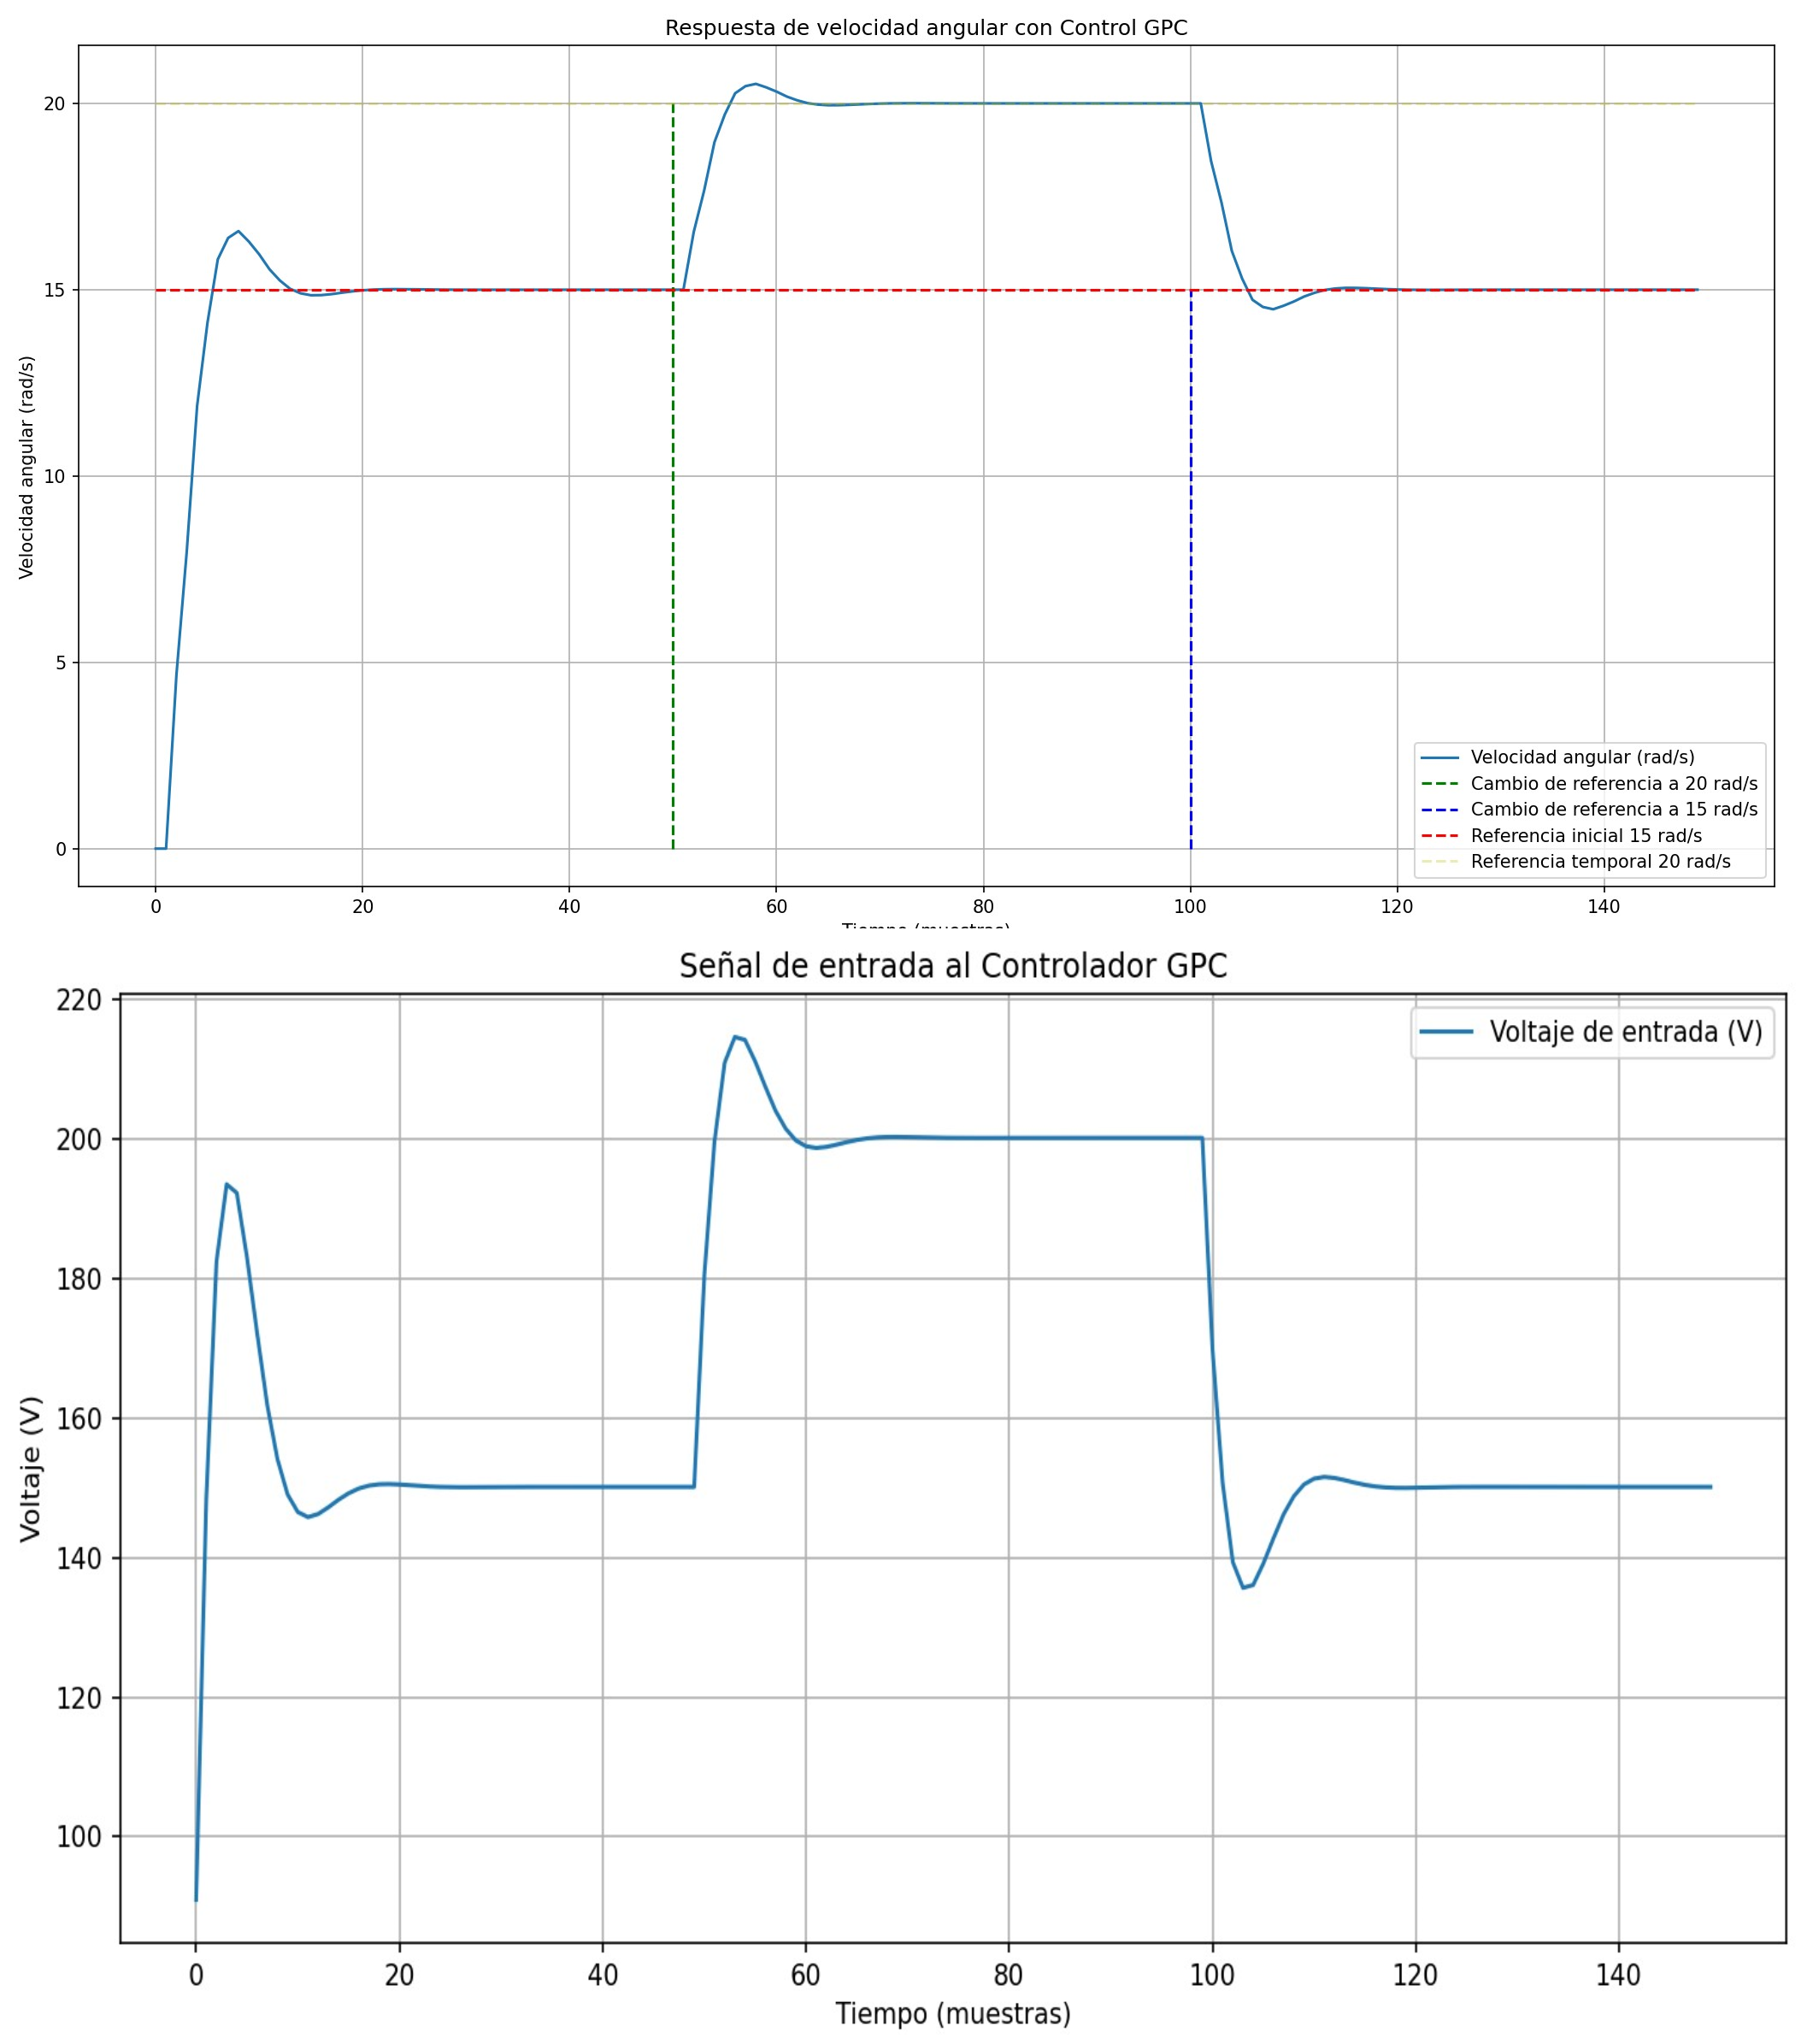
\includegraphics[width=\linewidth]{imagen-2-2.png}
                \caption{Respuesta de la velocidad angular en $[rad/seg]$.}
                \label{fig:practico-1}
            \end{figure}
        \end{column}
        
        % Columna derecha: Texto
        \begin{column}{0.5\textwidth}
            \scriptsize
            \begin{justify}
                En la implementación y sintonización de un controlador predictivo generalizado (GPC), la matriz de ponderación del error \( Q \) juega un papel crucial en el equilibrio entre la rapidez de la respuesta transitoria y la suavidad de la acción de control. 

                \vspace{0.2cm}
                En las Figuras, se observa que al incrementar los valores de los elementos de \( Q \), se impone una mayor penalización sobre el error de seguimiento. Esto se traduce en una respuesta más agresiva del controlador, buscando minimizar la desviación de la trayectoria deseada con mayor determinación. Como consecuencia directa, se observa una reducción en el tiempo de establecimiento del estado transitorio, entre la salida predicha y la trayectoria de referencia.

                \vspace{0.2cm}
                Además, un incremento significativo en los valores de Q puede introducir un comportamiento de sobreimpulso en la velocidad angular del sistema, donde se excede la referencia
establecida
            \end{justify}
        \end{column}
    \end{columns}
\end{frame}


\begin{frame}{Simulación y respuesta del modelo}
    \begin{columns}
        % Columna izquierda: Imagen
        \begin{column}{0.45\textwidth}
            \begin{figure}
                \centering
                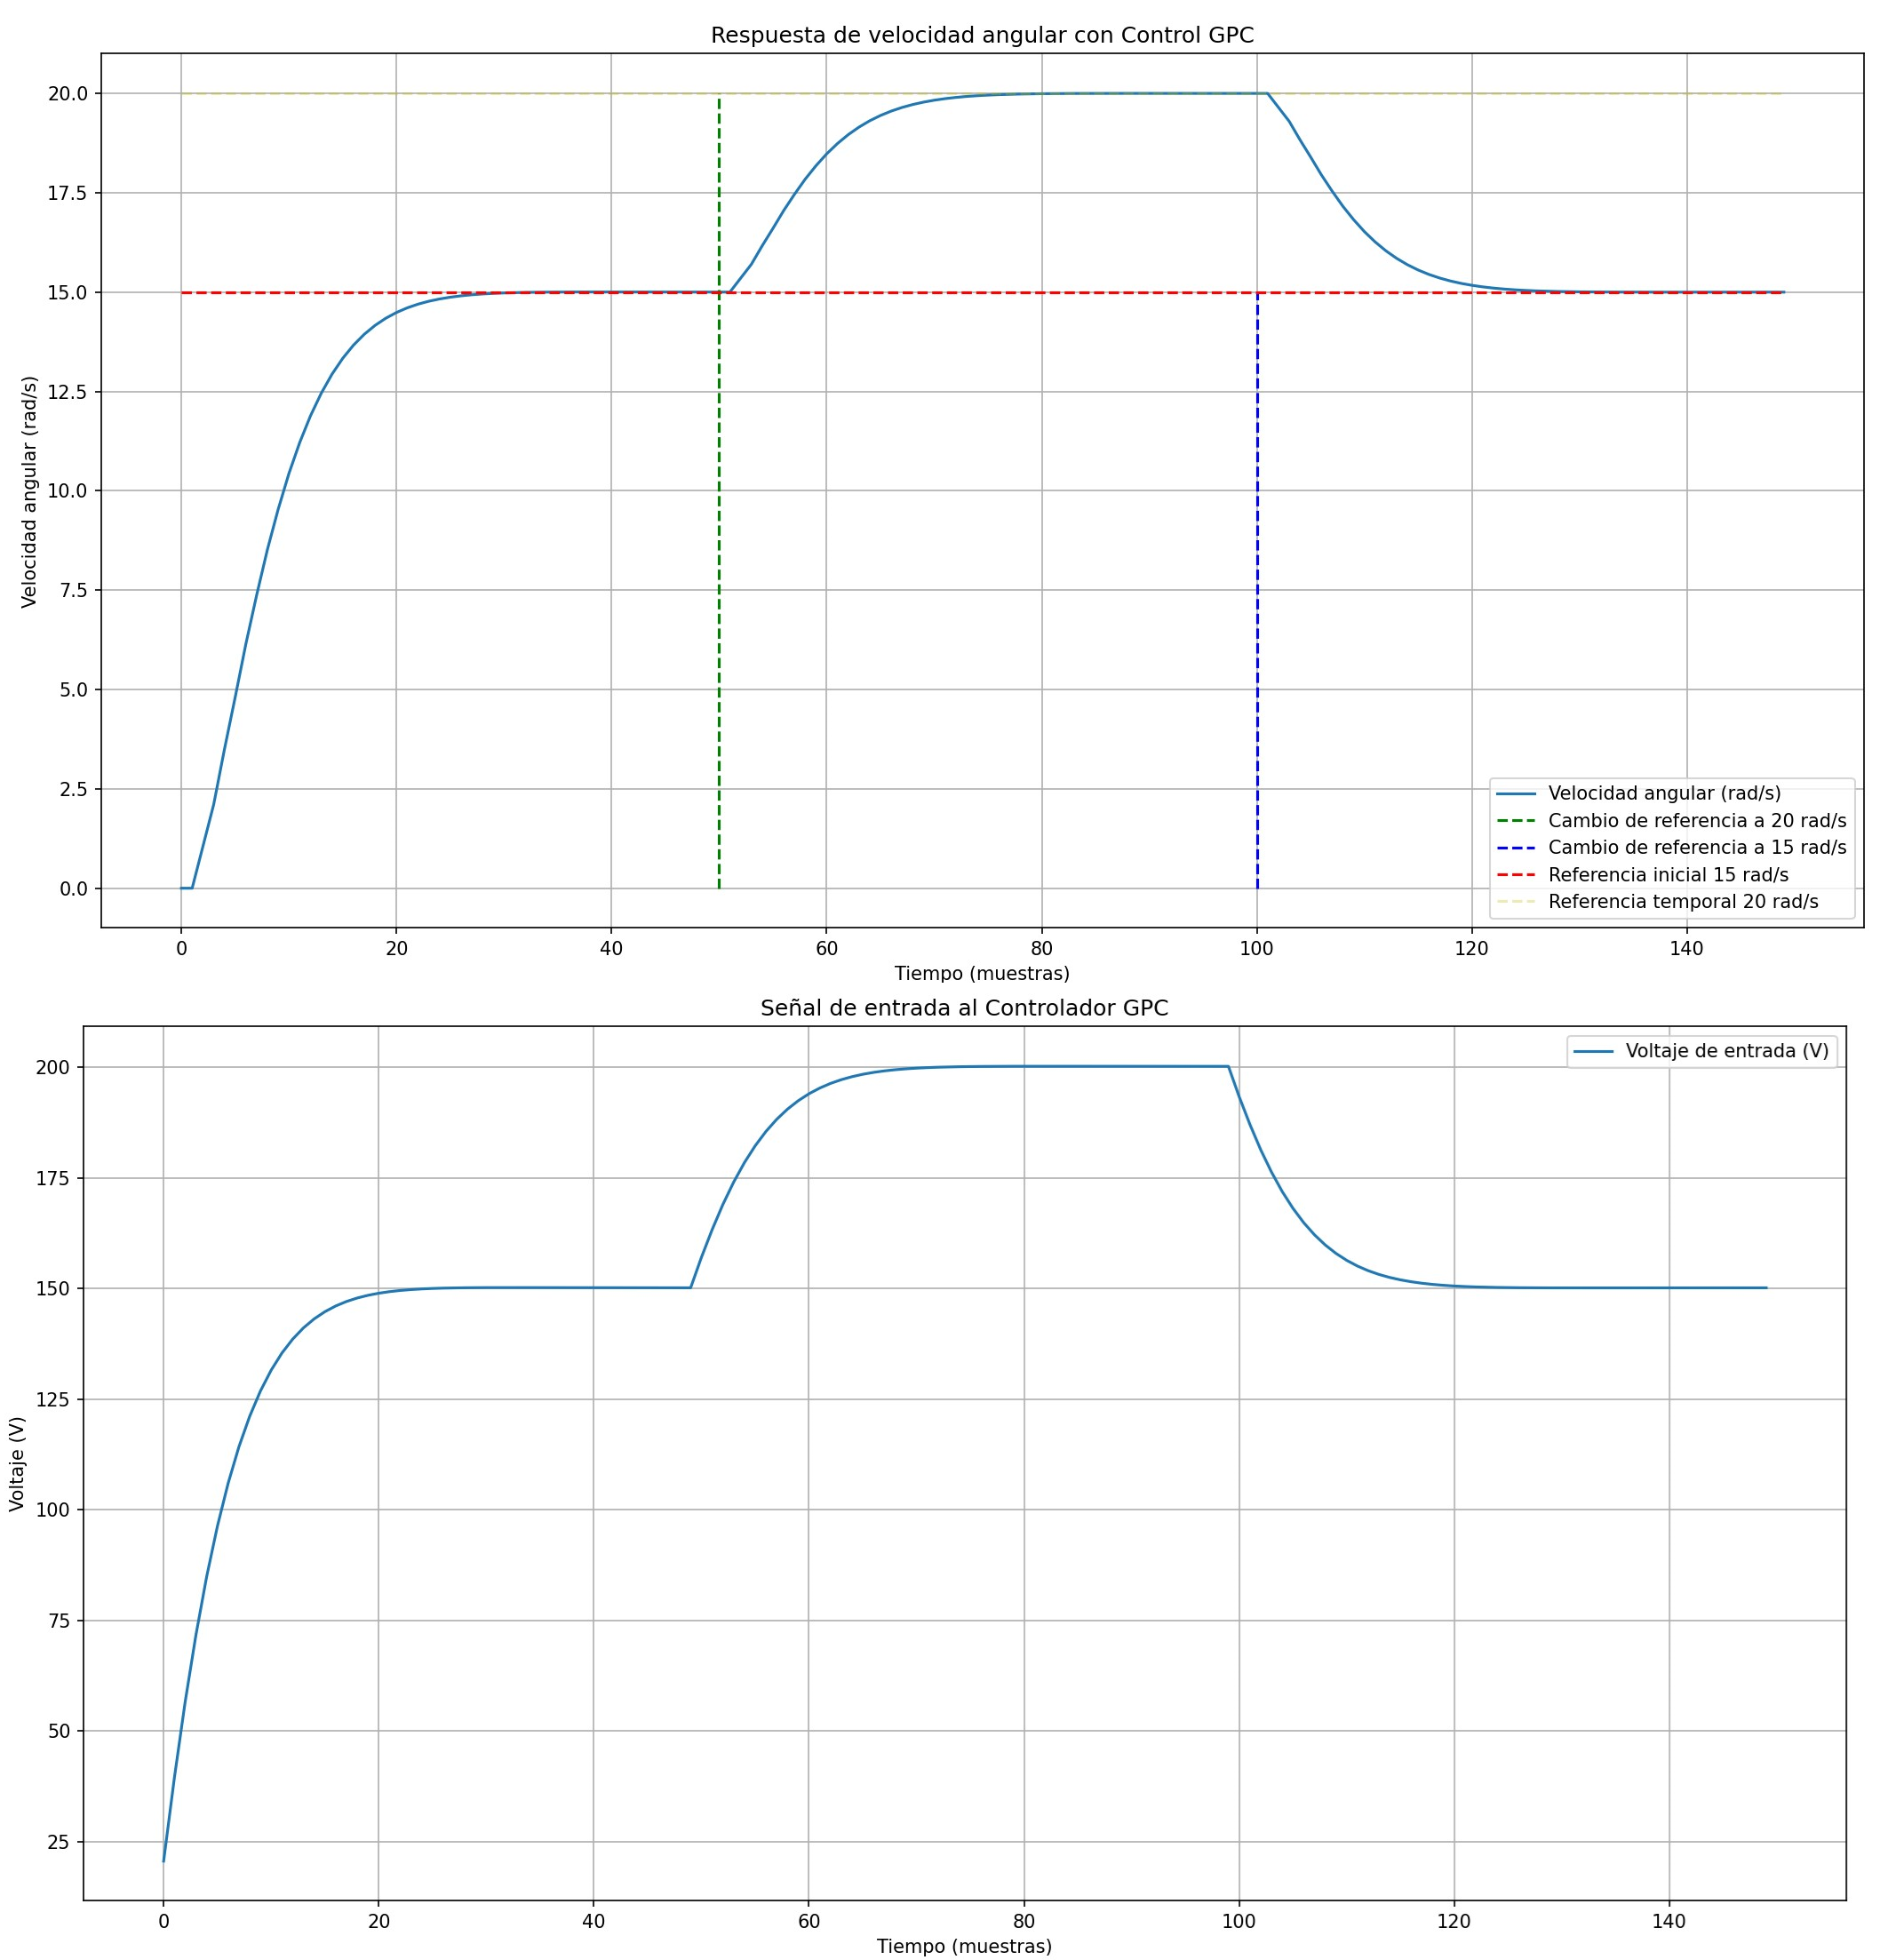
\includegraphics[width=\linewidth]{imagen-4-4.png}
                \caption{Respuesta de la velocidad angular en $[rad/seg]$.}
                \label{fig:practico-1}
            \end{figure}
        \end{column}
        
        % Columna derecha: Texto
        \begin{column}{0.5\textwidth}
            \scriptsize
            \begin{justify}
                Como se ilustra en las Figuras,  un incremento en los valores de los pesos asociados a la matriz \( R \) provoca una extensión en los periodos de estado transitorio, reflejando un aumento en el tiempo que la velocidad angular, medida en \([rad/s]\), requiere para alcanzar el estado estacionario. Este fenómeno se atribuye a que una mayor ponderación en \( R \) induce una respuesta más cautelosa del controlador, priorizando la suavidad de la señal de control sobre la rapidez de seguimiento de la referencia.

                Además, se observa que la señal de voltaje correspondiente al control de entrada adopta un perfil más suave. Esta característica es ventajosa en la práctica, ya que evita los sobreimpulsos en el voltaje que podrían ocasionar daños a los componentes electrónicos asociados al sistema de control.
            \end{justify}
        \end{column}
    \end{columns}
\end{frame}


\begin{frame}{Simulación y respuesta del modelo}
    \begin{columns}
        % Columna izquierda: Imagen
        \begin{column}{0.45\textwidth}
            \begin{figure}
                \centering
                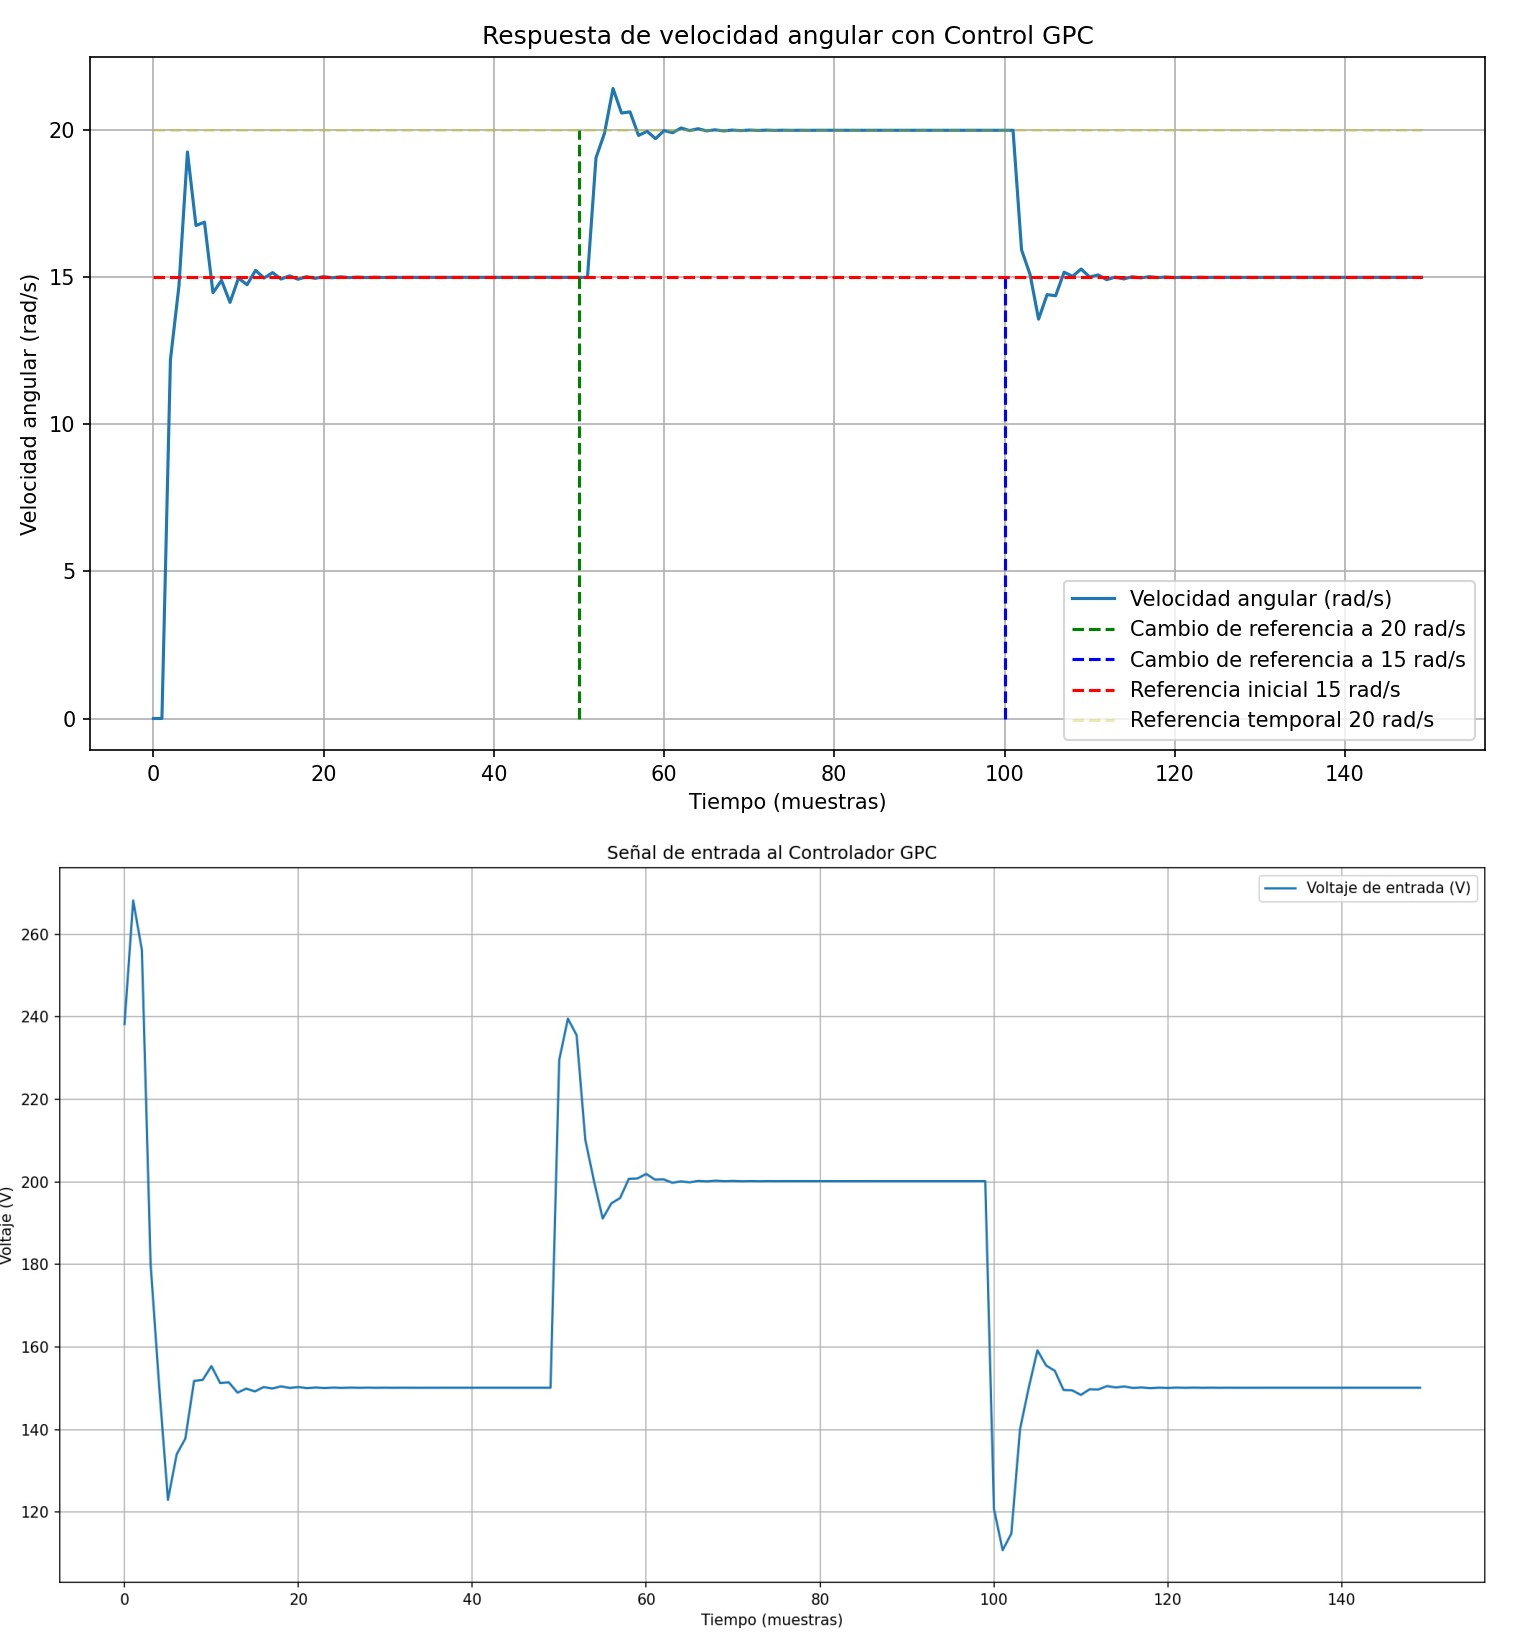
\includegraphics[width=\linewidth]{imagen-3-3.png}
                \caption{Respuesta de la velocidad angular en $[rad/seg]$.}
                \label{fig:practico-1}
            \end{figure}
        \end{column}
        
        % Columna derecha: Texto
        \begin{column}{0.5\textwidth}
            \scriptsize
            \begin{justify}
                Por otro lado, como se muestra en las Figuras, la reducción de los valores de los pesos \( R \) conduce a una disminución notable en los tiempos de estado transitorio, acompañada, sin embargo, de un sobreimpulso en la velocidad angular. Este comportamiento más agresivo en la respuesta del sistema se manifiesta a través de señales de control con oscilaciones y picos más pronunciados, que, si bien logran una estabilización más rápida, pueden ser perjudiciales para la integridad del motor y otros componentes mecánicos, especialmente si la entrada de control es el voltaje.

                \vspace{0.2cm}
                Este análisis describe la importancia de una cuidadosa selección de los valores dentro de la matriz \( R \) para el diseño del controlador predictivo generalizado (GPC). 
            \end{justify}
        \end{column}
    \end{columns}
\end{frame}




\begin{frame}{Comparación de los modelos con trabajo de referencia}
\begin{justify}
\vspace{0.3cm}

\begin{itemize}  
Comparando los resultados del control Propuesto y los del trabajo de Abdelrauf et al [1]:      
\begin{table}[ht]
  \centering
  \begin{tabular}{|c|c|}
    \hline
    Modelo GPC & Referencia PID \\
    \hline
    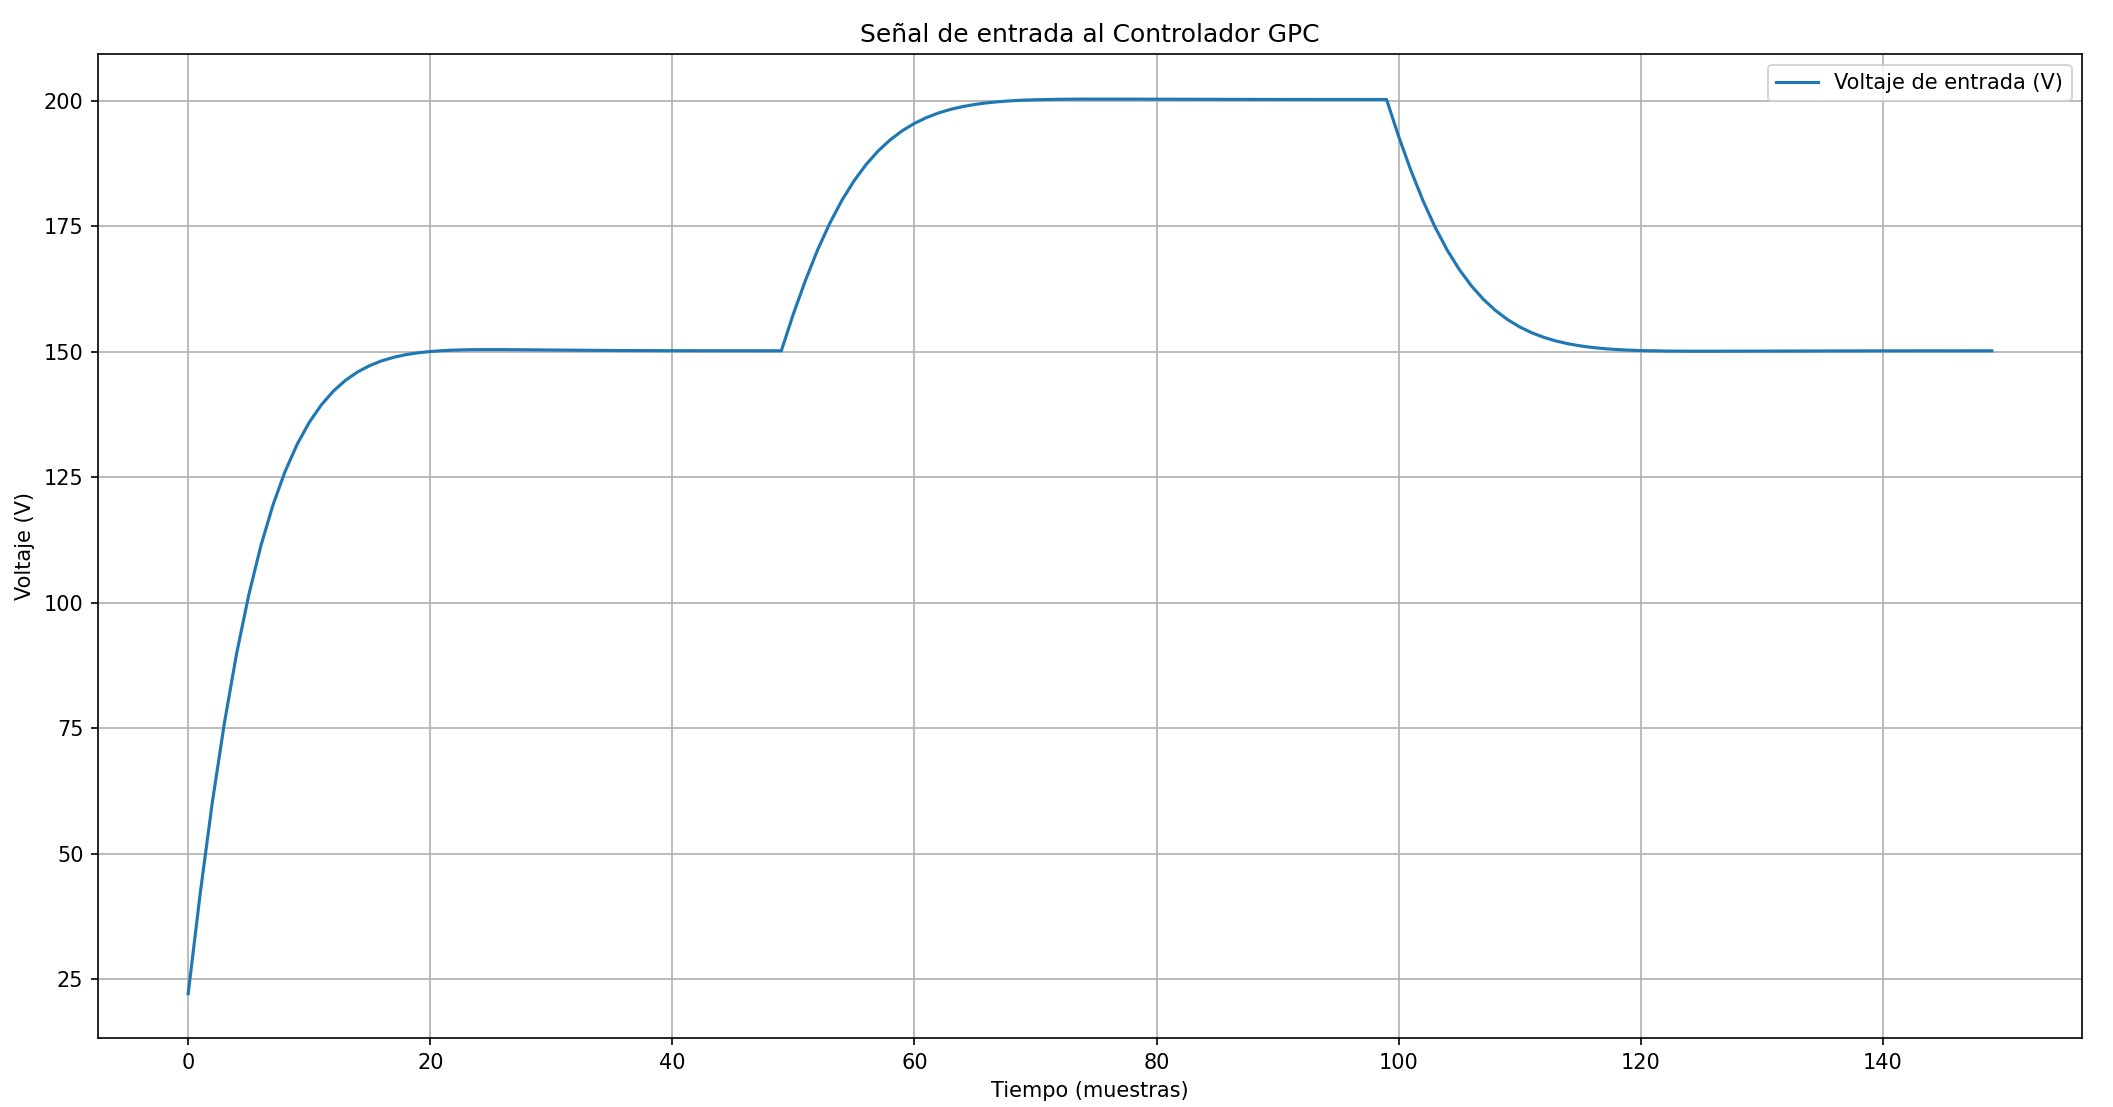
\includegraphics[width=0.4\linewidth]{imagen_2.png} & 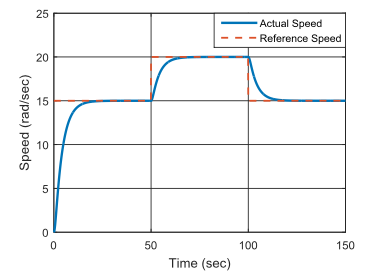
\includegraphics[width=0.45\linewidth, height=2.5cm]{RefPIDVolt.png} \\
    \hline
  \end{tabular}
  \caption{Comportamiento Voltaje (v) para un motor DC}
  \label{tab:tabla_con_imagenes}
\end{table}

\end{itemize}
\end{justify}
\end{frame}

\begin{frame}{Comparación de los modelos con trabajo de referencia}
\begin{justify}
\vspace{0.3cm}
\begin{itemize}  
Comparando los resultados del control Propuesto y los del trabajo de Abdelrauf et al [1]: 
\begin{table}[ht]
  \centering
  \begin{tabular}{|c|c|}
    \hline
    Modelo GPC & Referencia PID \\
    \hline
    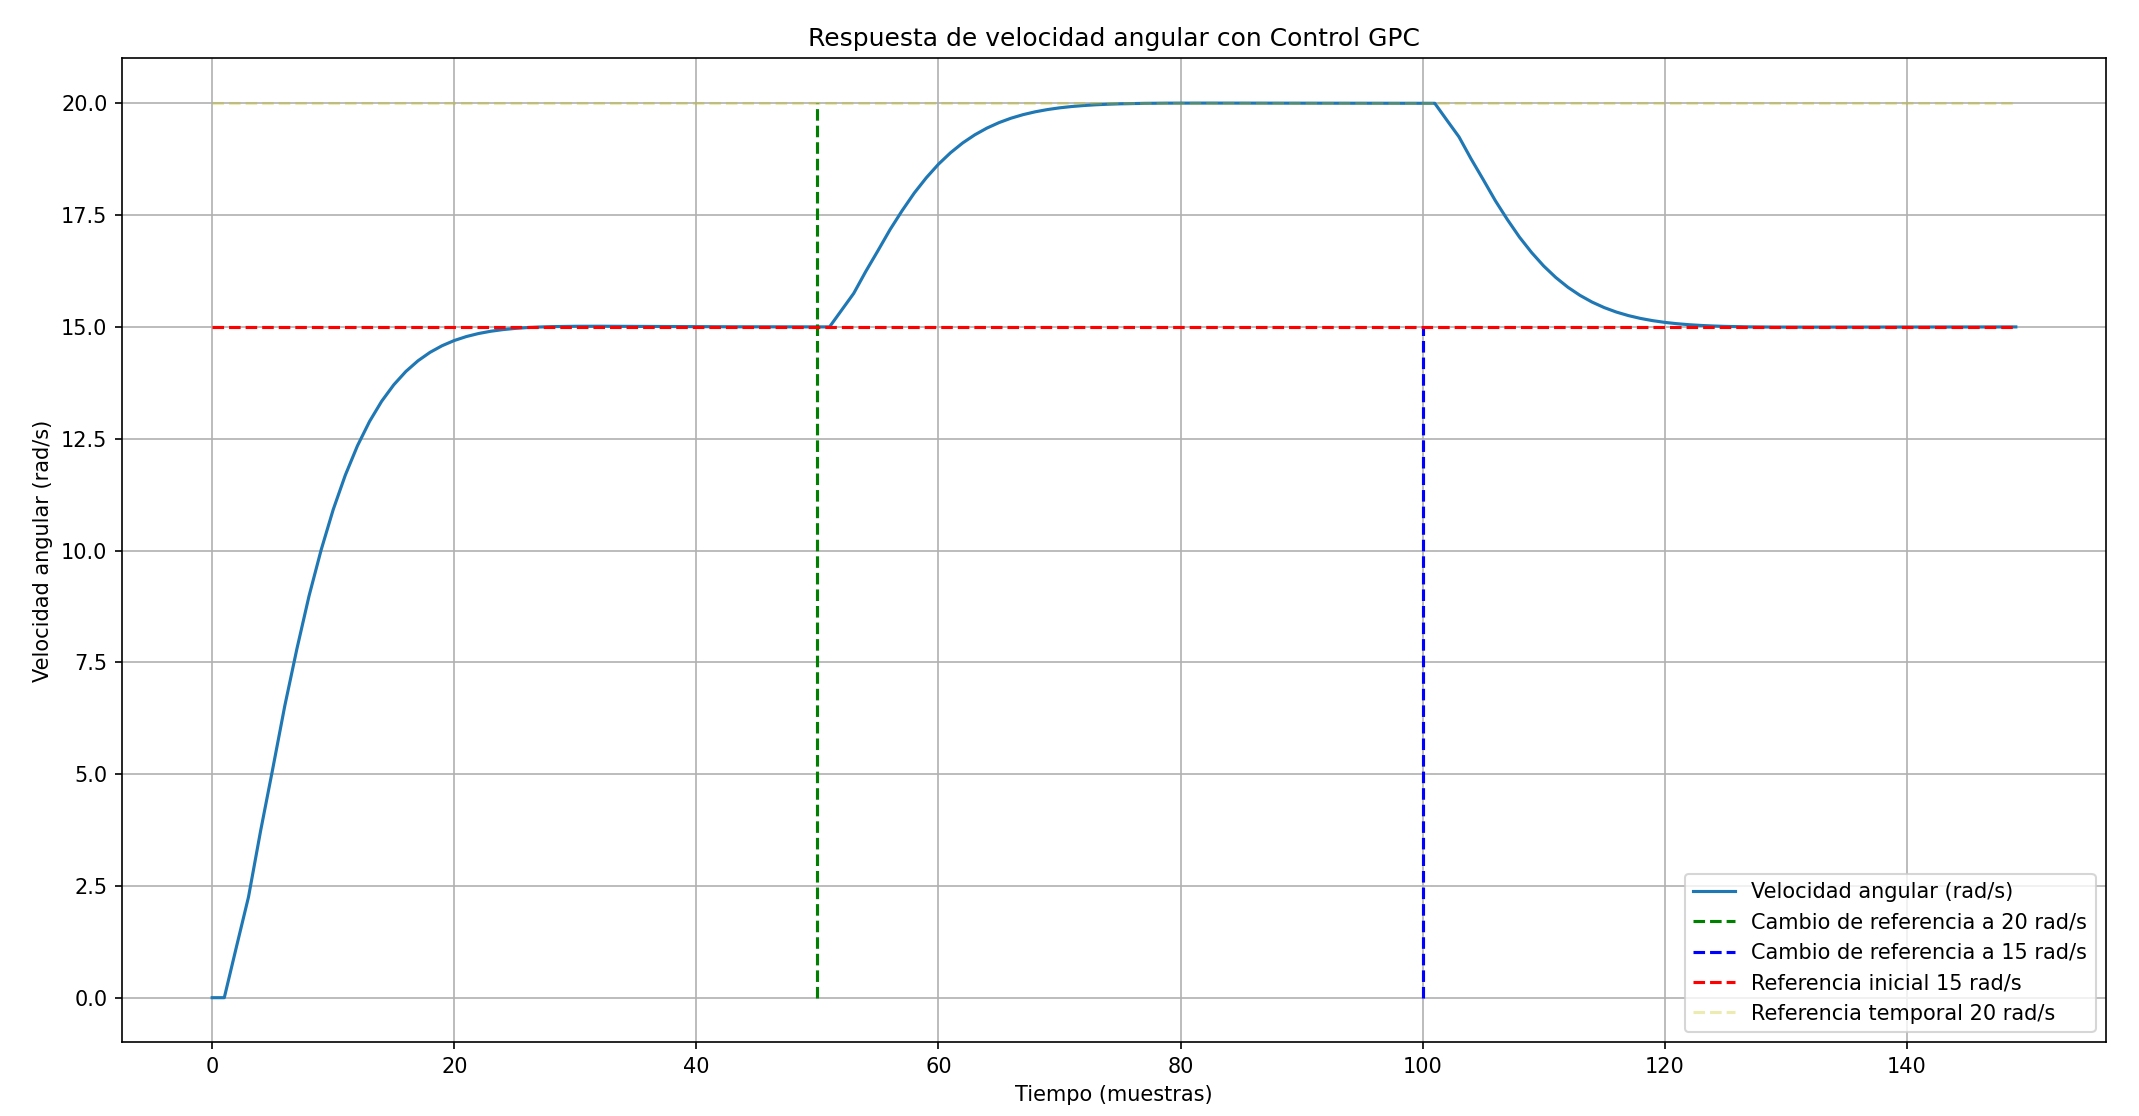
\includegraphics[width=0.4\linewidth]{imagen_1.png} & 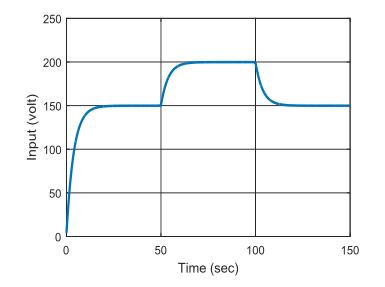
\includegraphics[width=0.45\linewidth, height=2.5cm]{RefPIDVel.png} \\
    \hline
  \end{tabular}
  \caption{Comportamiento de la velocidad angular para un motor DC}
  \label{tab:tabla_con_imagenes}
\end{table}
\end{itemize}
\end{justify}
\end{frame}

\begin{frame}{Conclusiones}
\begin{justify}
\vspace{0.3cm}
\begin{itemize}  
Este análisis describe la importancia de una cuidadosa selección de los valores dentro de la matriz \( R \) para el diseño del controlador predictivo generalizado (GPC). Ajustar adecuadamente \( R \) permite encontrar un equilibrio entre la protección de los componentes eléctricos y la eficiencia en la respuesta dinámica del sistema, factores ambos críticos para el funcionamiento seguro y efectivo en aplicaciones prácticas.
\end{itemize}
\end{justify}
\end{frame}

\begin{frame}{Conclusiones}
\begin{justify}
\vspace{0.3cm}
\begin{itemize}  
   En el presente trabajo se logró desarrollar una estrategia de control GPC para un motor DC. La selección cuidadosa y el ajuste fino de las matrices de ponderación de error \( Q \) y control \( R \) son esenciales para lograr una respuesta de control equilibrada. Es imperativo considerar la interacción entre \( Q \) y \( R \) para garantizar que se alcancen los objetivos de desempeño sin incurrir en comportamientos indeseables que puedan afectar adversamente al sistema o al proceso bajo control.
\end{itemize}
\end{justify}
\end{frame}

\begin{frame}{Referencias}
\begin{justify}
\vspace{0.3cm}
\begin{itemize}  
\\
(1)  A. A. Abdelrauf, M. Abdel-Geliel and E. Zakzouk, "Adaptive PID controller based on model predictive control," 2016 European Control Conference (ECC), Aalborg, Denmark, 2016, pp. 746-751, doi: 10.1109 /ECC.2016.7810378.
\\
(2) Huang, S. "Applied predictive control". 2002, Springer. 
\\
(3) S. Castanio, "Modelo de motor DC, Control Automático Educación", 22 de noviembre de 2023. https://controlautomaticoeducacion.com/analisis-de-sistemas/modelo-de-motor-dc/
\end{itemize}
\end{justify}
\end{frame}

\end{document}